\chapter{Metodología}
\thispagestyle{fancy}

\fancyhead[LE]{\thechapter.Metodología} 
La metodología es un factor muy importante de este proyecto, es la hoja de ruta a seguir, y por ello hay que definirla con precisión y saber cuál es la más apropiada.

\section{Consideraciones}
Debido a los objetivos mencionados en el apartado anterior, queda claro que existen varios tipos de objetivos en el proyecto. La metodología deberá ayudar a cumplir todos los objetivos específicos, para de esta manera, cumplir los objetivos generales. Sin embargo, dentro de los objetivos específicos se puede observar que coexisten tres tipos diferentes: de desarrollo, de investigación y de estudio.
\\ \\
Es difícil utilizar una misma metodología para el correcto desarrollo de los tres objetivos, ya que pertenecen a distintas disciplinas, así pues, se ha optado por combinar distintas metodologías para ello. De esta forma, se consigue conducir todos los objetivos en una misma dirección. Las metodologías que se combinarán serán:
\begin{itemize}
    \item \textbf{Metodología Cuantitativa}, metodología de investigación.
    \item \textbf{Modelo espiral}, metodología de desarrollo de software.
\end{itemize}

\section{Metodología de Investigación}
La metodología cuantitativa es una metodología de investigación que se centra en la recopilación y el análisis de los datos, lo que servirá como guía para los objetivos de estudio y el análisis de los resultados de los experimentos. 
\\ \\
Esta metodología declara que se deben llevar a cabo varias fases, sin embargo, solo se realizarán las siguientes tres:
\begin{enumerate}
    \item Definir claramente el problema y lo que se quiere hacer. 
    \item Delimitar el problema, concretar el alcance de la investigación.
    \item Revisión de la literatura, buscar los conocimientos necesarios para realizar el estudio.
\end{enumerate}
Después de haber realizado las tres fases de la metodología de la investigación, se aplicará la investigación empírica al estudio, la cual encaja perfectamente con el planteamiento de este proyecto. Esta forma de investigación es una forma de obtener conocimiento a través de la observación o experiencia. Además, mediante este método se incita a probar distintos experimentos y modificaciones con el objetivo de encontrar resultados diferentes.
\\ \\
Para aplicar esta metodología se usará el Ciclo empírico de A.D. de Groot (Fig.\ref{fig:CicloEmpirico}). Este ciclo ayuda a ordenar y entender las fases del proyecto, a conocer los siguientes pasos y a no perderse.
\\ \\
En el primer paso se encuentra la observación. Como el alumno ya ha adquirido la formación en el apartado tres de la metodología cuantitativa, podrá empezar observando cómo funciona el RS. A medida que se den más vueltas al modelo, esta observación se realizará sobre los resultados de los experimentos a la hora de aplicar FL.
\\ \\
En el segundo paso, el de inducción, se plantean las ideas o hipótesis acerca del paso de observación. En la primera vuelta, estas hipótesis e ideas serán sobre lo que ha aprendido el alumno y sobre cómo se aplicará el FL al proyecto. En las demás vueltas serán sobre los resultados observados y cómo estos afectan al proyecto y al estudio y qué mejoras podrían realizarse. 
\\ \\
Tanto la fase de deducción, donde se formulan los experimentos y pruebas a realizar, como la de pruebas, donde se realizan los experimentos para probar las hipótesis y recopilar datos, se sustituirán por la metodología de desarrollo de software en espiral. De esta forma, el modelo del ciclo empírico quedaría combinado con el de espiral para que la investigación y los experimentos que se están realizando mediante software sean concretos y tengan una correcta gestión (véase fig.\ref{fig:MetodologiaCombinada}). 
\\ \\
En el paso de evaluación, se interpretan los resultados de los experimentos de los anteriores dos pasos. En este apartado se hará un gran uso de  la estadística para mostrar la información, tanto gráfica como analiticamente.
\\ \\
Se pueden realizar tantas vueltas al ciclo empírico como sean necesarias.
\begin{figure}[thbp]
    \centering
    \fbox{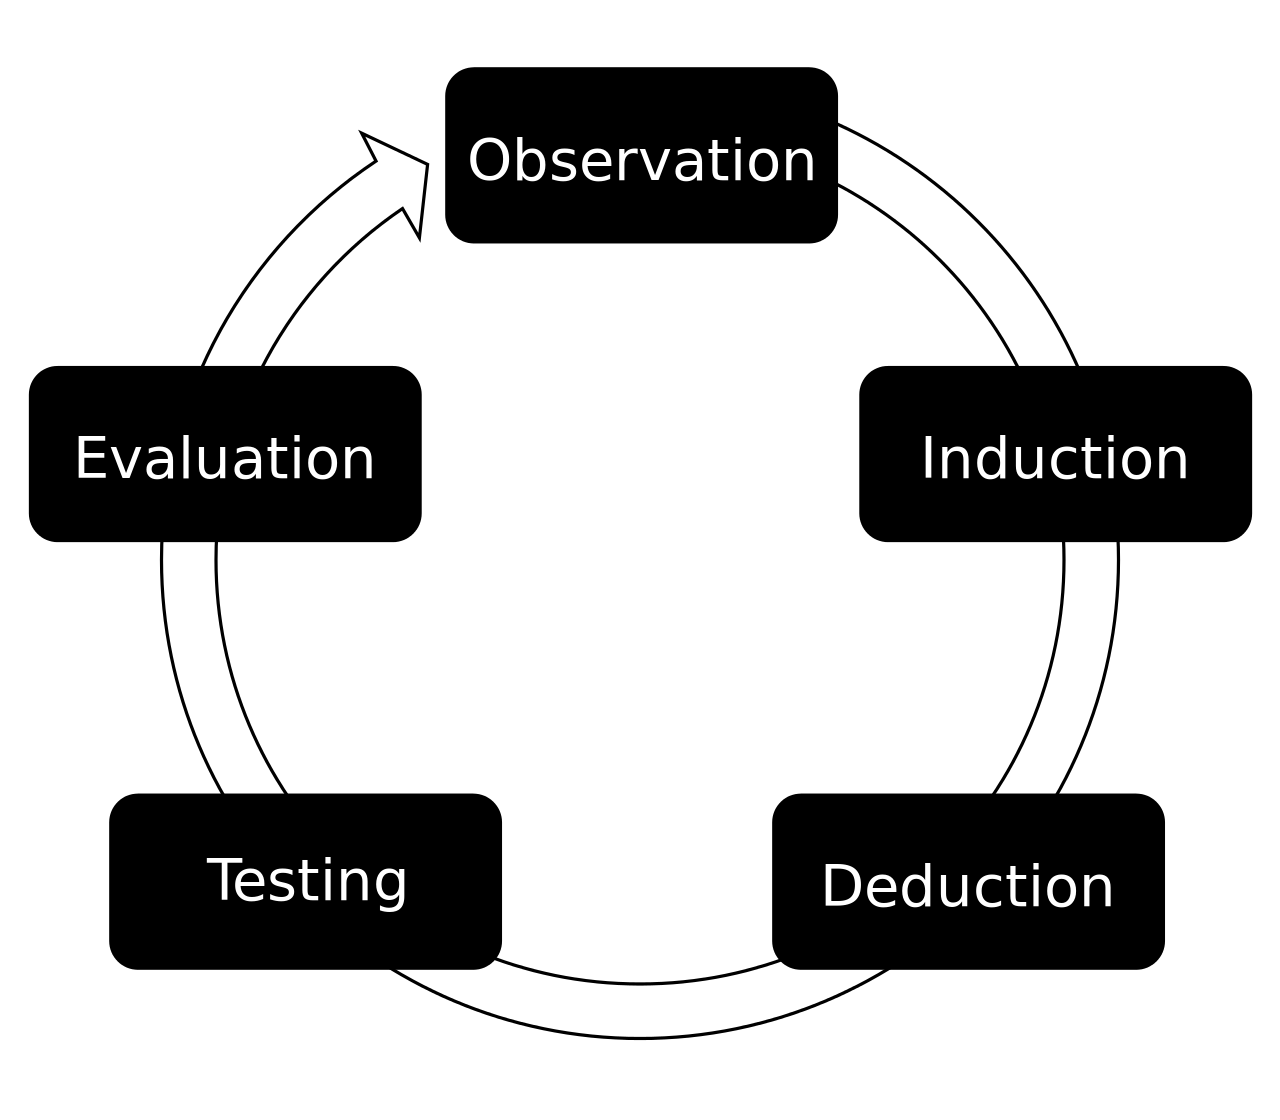
\includegraphics[width=0.45\textwidth]{Figuras/MetodologiaEmpirica.png}}
    \caption{Ciclo empírico de A.D. de Groot (Fuente: Wikipedia\autocite{InvestigacionEmpirica2020})} 
    \label{fig:CicloEmpirico}
\end{figure}

\section{Metodología de desarrollo}

El modelo en espiral (Fig.\ref{fig:MetodologiaEspiral}) formará parte del ya mencionado Ciclo empírico y agrupará los pasos de formulación de los experimentos y su ejecución. Se ha optado por incluir esta metodología dentro de otra para detallar más profundamente cómo será el proceso de desarrollo de software derivado de la investigación realizada.
\\ \\
Se ha elegido este modelo entre otros por varias razones importantes:
\begin{itemize}
    \item Define claramente lo que es un ciclo completo, los pasos a dar y las tareas a realizar. También fija los objetivos al inicio de cada ciclo de la espiral, lo que unido al paso de inducción del ciclo empírico implica que se definen objetivos claros y concisos sobre las hipótesis planteadas.
    \item Al ser un modelo continuo, se pueden realizar tantas iteraciones sobre la espiral como se necesiten, permitiendo desarrollar tantos experimentos como hipótesis se plantean en el apartado de inducción del ciclo empírico. Además, cada vuelta de la espiral incluye el desarrollo de prototipos (lo que en este caso sería un experimento), que al contar con una fase de integración consigue que puedan coexistir todos en el mismo entorno de desarrollo.
    \item Cumple con las fases de Deducción y Testeo del ciclo empírico ya que incluye los pasos de estas en la fase de desarrollo de la espiral.
    \item Por último y más importante, se ha elegido esta metodología porque tiene en cuenta la gestión y análisis de riesgos. Esto tiene gran importancia al tratarse de un proyecto complejo con múltiples dispositivos y tanta cantidad de pruebas a realizar.
\end{itemize}

\begin{figure}[thbp]
    \centering
    \fbox{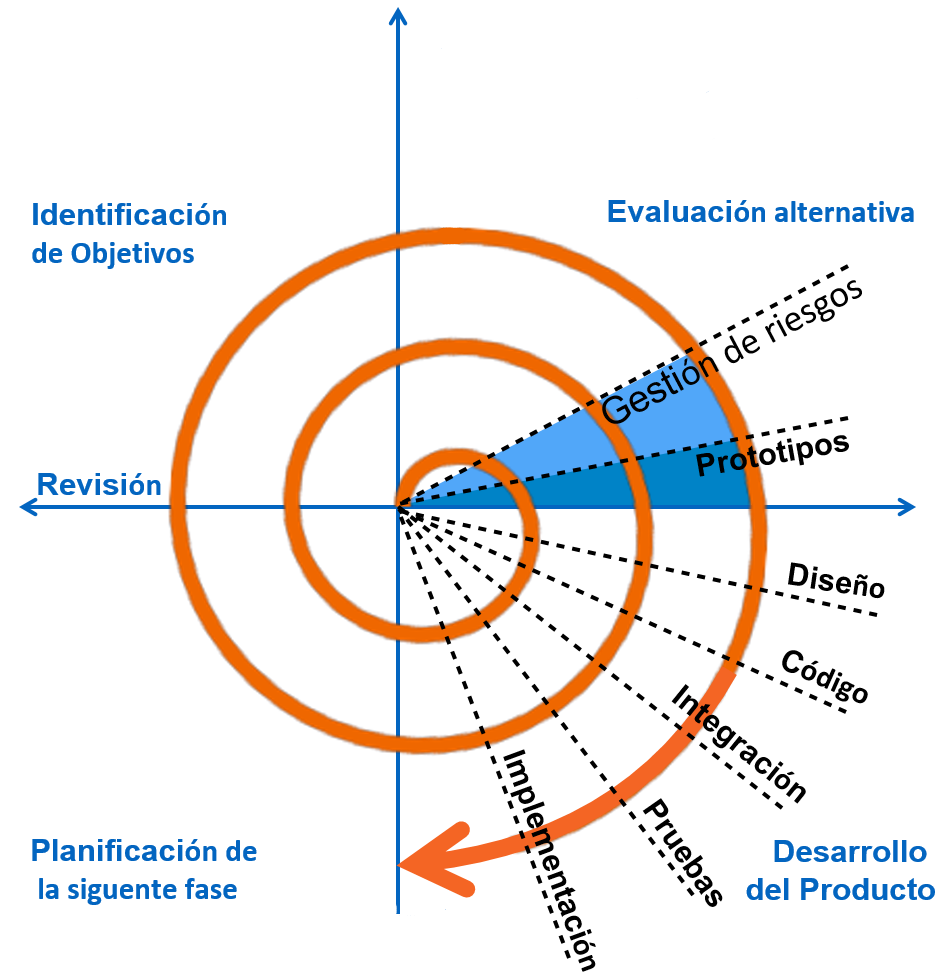
\includegraphics[width=0.6\textwidth]{Figuras/MetodologiaEspiral.png}}
    \caption{Modelo en el Espiral, Autor Desconocido (Fuente: Blog\autocite{CicloVidaSoftware2016})} 
    \label{fig:MetodologiaEspiral}
\end{figure}

\section{Conclusión}
Partiendo del ciclo empírico, escisión de la metodología de investigación cuantitativa, se hará especial hincapié en la continua reflexión y teorización sobre el modelo de FL implantado. 
\\ \\
Para el correcto desarrollo del software, las anteriormente mencionadas fases de deducción y testeo serán incluidas en el modelo de la espiral, consiguiendo así, una gestión eficiente y precisa sobre los pasos a dar tanto en investigación como en el desarrollo de software.
\\ \\
Como se ha comentado anteriormente, la agrupación de estas dos metodologías permitirá combinar la investigación con el desarrollo de software, descubriendo a base de prueba y error y a base de analizar los resultados las mejores soluciones para el RS basado en FL.
\\ \\
Por lo cual, una vez el alumno haya definido claramente el problema, su alcance y se haya formado en la tecnología, podrá comenzar a utilizar el ciclo presente en la figura \ref{fig:MetodologiaCombinada}.

\begin{figure}[thbp]
    \centering
    \fbox{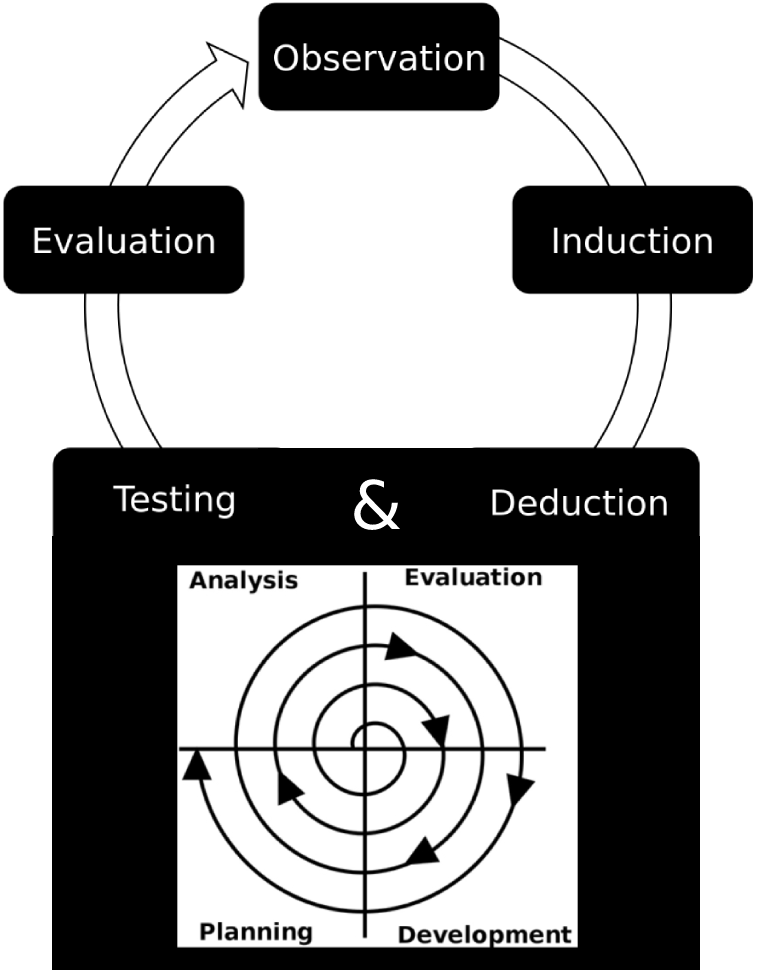
\includegraphics[width=0.6\textwidth]{Figuras/MetodologiaCombinada.png}}
    \caption{Metodología de trabajo del proyecto final de grado (Autor: Elaboración propia)} 
    \label{fig:MetodologiaCombinada}
\end{figure}